\documentclass[letterpaper,12pt]{article}
%\usepackage{harvard}
%\usepackage{subfigure}
%\usepackage[active]{srcltx}
\usepackage{graphicx}
\usepackage{pdflscape}
\usepackage{amsmath}
\usepackage{amsthm}
\usepackage{lscape}
\usepackage{enumerate}
\usepackage{float}
\usepackage{grffile}
\usepackage{relsize}
\usepackage{tablefootnote}
\usepackage{footnote}
\usepackage{sectsty}
\usepackage{xcolor}
\usepackage{caption}
\usepackage{color}
\usepackage{natbib}
\usepackage{multirow}
\usepackage{bbm}
\usepackage[T1]{fontenc}
\usepackage[multiple]{footmisc}
\usepackage{appendix}
\usepackage{times}
\usepackage{relsize}
\usepackage{caption}
\usepackage{newtxtext,newtxmath}
\usepackage{enumitem}


%%%%%%%%%%%%%%%%%%%%%%%%%%%%%%%%%%%%%%%%%%%%%%%%%%%%%%%%%%%%
%%%   Title Page Information
%%%%%%%%%%%%%%%%%%%%%%%%%%%%%%%%%%%%%%%%%%%%%%%%%%%%%%%%%%%%
\title{\vspace{-.4in} ECON311: Assignment II -- Solutions}
\author{Leandro Freylejer}
\date{}

%%%%%%%%%%%%%%%%%%%%%%%%%%%%%%%%%%%%%%%%%%%%%%%%%%%%%%%%%%%%
%%%   Double and Single Space Commands
%%%%%%%%%%%%%%%%%%%%%%%%%%%%%%%%%%%%%%%%%%%%%%%%%%%%%%%%%%%%
\newlength{\defbaselineskip}
\setlength{\defbaselineskip}{\baselineskip}
\newcommand{\setlinespacing}[1]{\setlength{\baselineskip}{#1 \defbaselineskip}}
\newcommand{\doublespacing}{\setlength{\baselineskip}{1.3 \defbaselineskip}}
\newcommand{\singlespacing}{\setlength{\baselineskip}{1\defbaselineskip}}
\renewcommand{\thesubsection}{\arabic{subsection}}
\newtheoremstyle{dotlessS}{}{}{\itshape}{}{\color{dg}\bfseries}{}{ }{}
\theoremstyle{dotlessS}
\newtheorem{theorem}{Theorem}
\newtheorem{lemma}{Lemma}
\newtheorem{proposition}{Proposition}
\newtheorem{assumption}[theorem]{Assumption}
\newtheorem{corollary}{Corollary}
\newtheorem{definition}{Definition}
\newenvironment{example}[1][Example]{\begin{trivlist}
\item[\hskip \labelsep {\bfseries #1}]}{\end{trivlist}}
\newenvironment{remark}[1][Remark]{\begin{trivlist}
\item[\hskip \labelsep {\bfseries #1}]}{\end{trivlist}}

\newcommand\Pitem{%
  \addtocounter{enumi}{-1}%
  \renewcommand\theenumi{\arabic{\enumi}'}%
  \item%
  \renewcommand\theenumi{\arabic{enumi}}%
}

%%%%%%%%%%%%%%%%%%%%%%%%%%%%%%%%%%%%%%%%%%%%%%%%%%%%%%%%%%%%
%%%   Set Margins Here
%%%%%%%%%%%%%%%%%%%%%%%%%%%%%%%%%%%%%%%%%%%%%%%%%%%%%%%%%
\textwidth=6.5in
\textheight=9in
\oddsidemargin=0.10in
\evensidemargin=0.10in
\topmargin=-0.5in
%\parskip=3pt

%%%%%%%%%%%%%%%%%%%%%%%%%%%%%%%%%%%%%%%%%%%%%%%%%%%%%%%%%%%%%
%%%   Actual Document Begins Here
%%%%%%%%%%%%%%%%%%%%%%%%%%%%%%%%%%%%%%%%%%%%%%%%%%%%%%%%%%%%%
\begin{document}
\pagenumbering{arabic}
\maketitle
\vspace{-.6in}

\section*{Question I: Long-Run Growth}
Consider the following Romer economy without capital: 
\begin{eqnarray*}
\begin{array}{ll}
\text{Production Function:} & Y_t=A_t \: L_{Y_t} \\[1.4ex]
\text{Law of Motion for Productivity:} & A_{t+1}=A_t+\overline{z} \: A_t \: L_{A_{t}}  \\[1.4ex]
\text{Allocation of labour:} & L_{A_{t}}=\overline{I} \: \overline{L}, \: \: \:  \: \: L_{Y_{t}}=(1-\overline{I}) \: \overline{L}  \\[1.4ex]
\end{array}
\end{eqnarray*}
\begin{enumerate}[label=(\alph*)]
\item (6 points) Derive the rate of growth of output per person ($g_{y}$, where $y=\frac{Y}{\overline{L}}$).\\
\\
\textbf{Answer:}\\

From the production function: \begin{eqnarray*}
									\begin{array}{l}										
									\frac{Y_t}{\overline{L}}=y_t=A_t (1-\overline{I})  \\
									g_y=g_A+g_{(1-\overline{I})}\\
                                            g_y=g_A
									\end{array}
								   \end{eqnarray*}
To calculate $g_A$, we use the law of motion for productivity:
\begin{eqnarray*}
\frac{A_{t+1}-A_t}{A_t}=g_A=\overline{z}\overline{I} \overline{L}=g_y
\end{eqnarray*}
									
\item (6 points) Assume two countries, country $1$ and country $2$, that are the same in every respect, except across two dimensions. First, assume that in the year $1950$, country $1$ has a larger level of output productivity ($A_{1950}^{\text{country 1}}> A_{1950}^{\text{country 2}}$). Second, assume that country $2$ is more productive in generating ideas ($\overline{z}^{\text{country 1}}<\overline{z}^{\text{country 2}}$). On the same graph draw the evolution of output per person over time for these two countries using a ratio scale and starting in the year 1950. Which country do you think will have larger output per person in the long run? Explain.  \\
\\
\textbf{Answer:}\\
In 1950: $\frac{Y^{country1}}{\overline{L}}=A^{country1}_{1950}(1-\overline{I})>A^{country2}_{1950}(1-\overline{I})=\frac{Y^{country2}}{\overline{L}}$ \\
However, $g_y^{country1}=\overline{z}^{country1}\overline{I} \overline{L}<\overline{z}^{country2}\overline{I} \overline{L}=g_y^{country2}$. Therefore, country 2's output per person will eventually be greater than country 1's.

\begin{figure}[H]
\centering
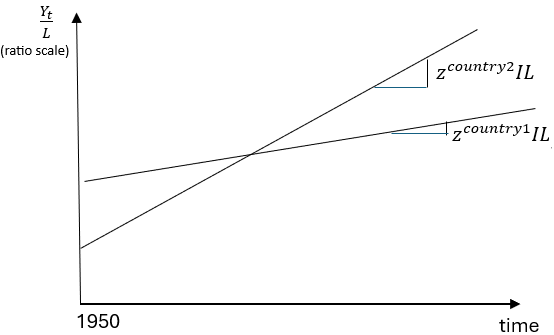
\includegraphics[scale=0.8]{growth}
\end{figure} 
\end{enumerate} 

\section*{Question II: IS-MP and Phillips Curve (10 points)}
Consider the following economy, which is the same economy as the one presented in class:
\begin{eqnarray*}
\begin{array}{ll}
\text{Aggregate Expenditure} &E_t=C_t+I_t+G_t+X_t-M_t \\[1.4ex]
\text{Consumption} &C_t=a_c+b_c Y_t \\[1.4ex]
\text{Investment} & I_t=a_i-b_i \: \: \: R_t \\[1.4ex]
\text{Inflation} &\pi_t=\pi_{t-1}+\overline{v} \: \: \: \widetilde{Y}_t+\overline{o}_t  \\[1.4ex]
\text{Government Expenditure and Trade} & G_t=\overline{G}, \: \: \: \: \: \: M_t=\overline{M}, \: \: \: \: \: \: X_t=\overline{X}
\end{array}
\end{eqnarray*}
Suppose that this economy is at its long-run equilibrium, with $\overline{o}_t=0 $ and $\pi_t=0.06$. Assume that the government wants to decrease the level of inflation to $\pi_{t+3}=0.03$. To do that they decided to use Monetary Policy ($R_t$) to reduce $\pi$ by 0.01 each year for three years. Using the full short-run model (IS-MP and Phillips curve), explain what happens to the economy \textbf{over time}. Be sure to include graphs showing: i. the IS-MP, ii. the Phillips Curve, and iii. how deviations from potential output and the level of inflation respond over time. Carefully label all graphs (including the level of potential output as a  function of parameters and the change in inflation in each period).\\
\\
\textbf{Answer:}\\
\\
To decrease inflation the government increases the interest rate from its long-run level, $\overline{r}$, to $R_t$, where $R_t> \overline{r}$, for three consecutive periods: $t=\tau+1$,$\tau+2$, and $\tau+3$. This results in a decrease of $\widetilde{Y}_t$ over the same time period.  From the Phillips Curve, we know that, at $t=\tau+1$,$\tau+2$, and $\tau+3$:
\begin{eqnarray*}
\begin{array}{lll}
-0.01=\overline{v} \: \widetilde{Y}_t    &  \Rightarrow  & \widetilde{Y}_t=-\frac{0.01}{\overline{v}}
\end{array}
\end{eqnarray*}
The IS-MP, Phillips Curve, and the Dynamics of $\widetilde{Y}_t$ and $\Pi_t$ graphs are as follows:
\begin{figure}[H]
\centering
\caption*{$\: \: \: \: \: $ IS and MP Curves }
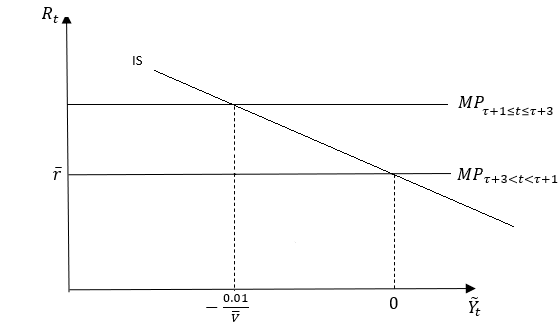
\includegraphics[scale=1]{nq_1}
\end{figure}

\begin{figure}[H]
\centering
\caption*{$\: \: \: \: \: $ Phillips Curve }
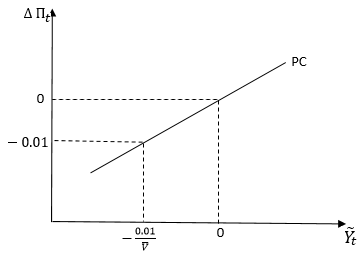
\includegraphics[scale=1.3]{nq_1_PC}
\end{figure}

\begin{figure}[H]
\centering
\caption*{$\: \: \: \: \: $ Time Graphs }
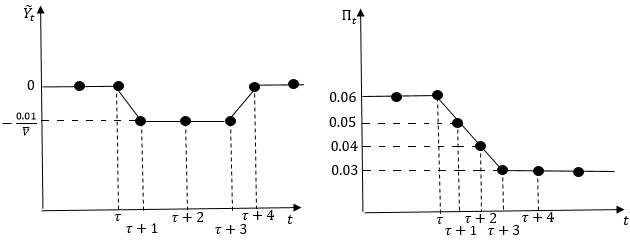
\includegraphics[scale=1.1]{nq_1_time_graphs}
\end{figure}





\section*{Question III: Keynesian Cross, IS-MP and Phillips Curve}
Consider the following economy:
\begin{eqnarray*}
\begin{array}{ll}
\text{Aggregate Expenditure} &E_t=C_t+I_t+G_t+X_t-M_t \\[1.4ex]
\text{Consumption} &C_t=a_c+b_c (Y_t-T_t) \\[1.4ex]
\text{Investment} & I_t=a_i-b_i \: \: \: R_t \\[1.4ex]
\text{Taxes} &T_t=b_T \: \: \: Y_t  \\[1.4ex]
\text{Inflation} &\pi_t=\pi_{t-1}+\overline{v} \: \: \: \widetilde{Y}_t+\overline{o}_t  \\[1.4ex]
\text{Government Expenditure and Trade} & G_t=\overline{G}, \: \: \: \: \: \: M_t=\overline{M}, \: \: \: \: \: \: X_t=\overline{X}
\end{array}
\end{eqnarray*}
In this economy, taxes depend on the level of income. Moreover, consumption depends on disposable income (income net of taxes) and not just on the level of income as we assumed in class. Use the previous equations to answer the following questions:
\begin{enumerate}[label=(\alph*)]
\item (4 points) Solve for the equilibrium in the goods market. What is the expenditure multiplier? \\
\\
\textbf{Answer:}\\
\begin{eqnarray*}
\begin{array}{l}
E_t=a_c+b_c \: Y_t-b_c \: b_T \: Y_t+a_i-b_i \: R_t+\overline{G}+\overline{X}-\overline{M} \\
E_t=\left[a_c+a_i-b_i \: R_t+\overline{G}+\overline{X}-\overline{M}\right]+ \: \left[b_c-b_c \: b_T\right] \: Y_t \\
\end{array}
\end{eqnarray*}
In equilibrium, $Y_t=E_t$. Solving for $Y_t$:
\begin{eqnarray*}
Y_t=\underbrace{\frac{1}{1-b_c+b_c \: b_T}}_{\text{multiplier}}\left[a_c+a_i-b_i \: R_t +\overline{G}+\overline{X}-\overline{M}\right]
\end{eqnarray*}
\item (7 points) Use the Keynesian Cross to carefully explain the effect of a positive shock to the government expenditure, $\overline{G}$, for two cases: i. $b_T<1$, ii. $b_T=1$  (carefully label both graphs, including the slope of the expenditure function).  What is the assumption we need to make to guarantee an equilibrium exists?\\
\\
\textbf{Answer:}\\
Assumption: $(b_c-b_c \: b_T)<1$. There are two cases shown below
\begin{itemize}
\item $b_T<1 \Rightarrow b_c-b_c \: b_T>0$
\begin{figure}[H]
\centering
\caption*{$\: \: \: \: \: $ Keynessian Cross}
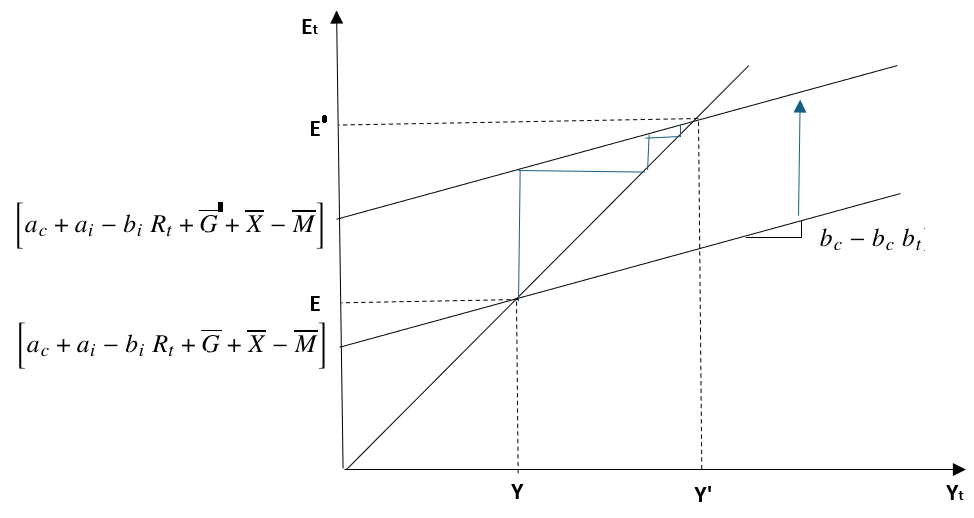
\includegraphics[scale=0.5]{k_cross}
\end{figure}
When $\overline{G}$ increases to $\overline{G}'$, the entire expenditure function shifts up. As the level of expenditure increases, so does output. The increase in output causes an additional increase in the level of expenditure, which again causes another increase in output. This feedback effect continues until it reaches the new equilibrium.
\item $b_T=1 \Rightarrow b_c-b_c \: b_T=0$
\begin{figure}[H]
\centering
\caption*{$\: \: \: \: \: $ Keynessian Cross}
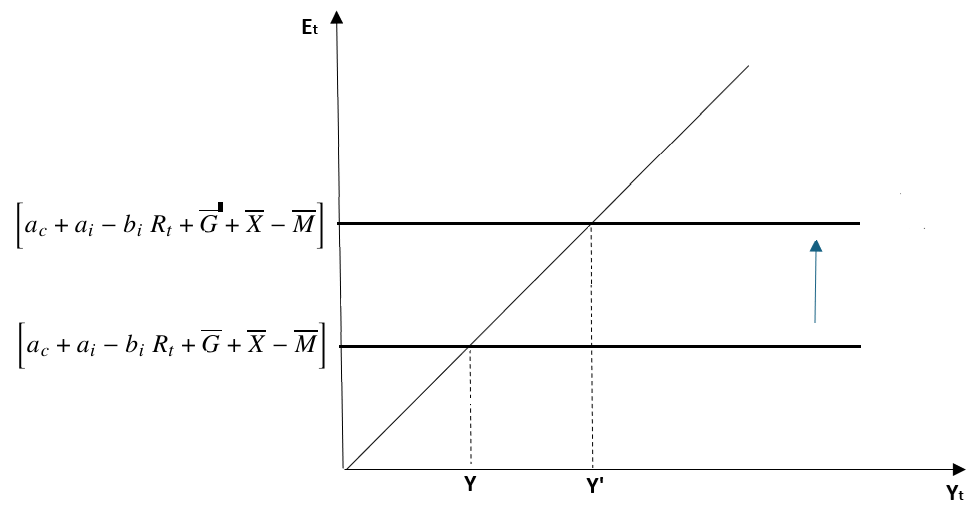
\includegraphics[scale=0.5]{k_cross2}
\end{figure}
In this case, the increase in expenditure causes $Y_t$ to increase by the same amount. The multiplier is 1. 
\end{itemize}

\item (4 points) Derive the IS curve using deviations from potential output as the endogenous variable.\\
\\
\textbf{Answer:}\\
Let $x=b_c-b_c \: b_T$, then
\begin{eqnarray*}
\begin{array}{l}
\frac{Y_t}{\overline{Y}}=\frac{1}{1-x}\left[\frac{a_c}{\overline{Y}}+\frac{a_i}{\overline{Y}}-\frac{b_i \: R_t}{\overline{Y}}+\frac{b_i \: \overline{r}}{\overline{Y}}-\frac{b_i \: \overline{r}}{\overline{Y}}+\frac{\overline{G}}{\overline{Y}}+\frac{\overline{X}}{\overline{Y}}-\frac{\overline{M}}{\overline{Y}}\right] \\[3ex]
\widetilde{Y}_t=\frac{1}{1-x}\left[\overline{a}-\overline{b}_i \: (R_t-\overline{r})\right]-1  \\[3ex]
\text{where   } \overline{a}=\frac{a_c+a_i-b_i \: \overline{r}+\overline{G}+\overline{X}-\overline{M}}{\underbrace{\frac{1}{1-x} \left[a_c^{LR}+a_i^{LR}-b_i \: \overline{r}+\overline{G}^{LR}+\overline{X}^{LR}-\overline{M}^{LR}\right]}_{\overline{Y}}}
\end{array}
\end{eqnarray*}

\item (9 points) Suppose the economy is at its potential output equilibrium with a constant $2\%$ inflation rate. Using the full short-run model (IS-MP and Phillips curve), explain what happens to the economy \textbf{over time} if the government decides to increase the level of expenditure for two periods. Be sure to include graphs showing how deviations from potential output and inflation respond over time.\\
\\
\textbf{Answer:}\\
Let the shock happens at $t=\tau$ and $t=\tau+1$, then
\begin{eqnarray*}
\begin{array}{ll}
IS-MP: & \widetilde{Y}_t=\left(\frac{1}{1-x} \overline{a}'\right)-1  \: \: \text{for    }  \: \: t=\tau, t=\tau+1 \\[3ex]
where, & \overline{a}'=\frac{1}{\overline{Y}}\left[a_c+a_i-b_i \: \overline{r}+\overline{G}'+\overline{X}-\overline{M}\right]>(1-x) \\
\end{array}
\end{eqnarray*}
\begin{figure}[H]
\centering
\caption*{$\: \: \: \: \: $ IS-MP}
\includegraphics[scale=0.5]{g_shock}
\end{figure}
\begin{eqnarray*}
\begin{array}{ll}
PC: & \Delta \Pi_t=\overline{V}\left[\frac{1}{1-x}\overline{a}'-1\right]  \: \: \text{for    }  \: \: t=\tau, t=\tau+1 \\[3ex]
where, &  \Delta \Pi_t=0 \: \: \text{for    }  \: \: t\neq\tau,\tau+1 \\[3ex]
\end{array}
\end{eqnarray*}
\begin{figure}[H]
\centering
\caption*{$\: \: \: \: \: $ Phillips Curve}
\includegraphics[scale=0.6]{phil}
\end{figure}
\begin{figure}[H]
\centering
\caption*{$\: \: \: \: \: $ Deviations from Potential Output}
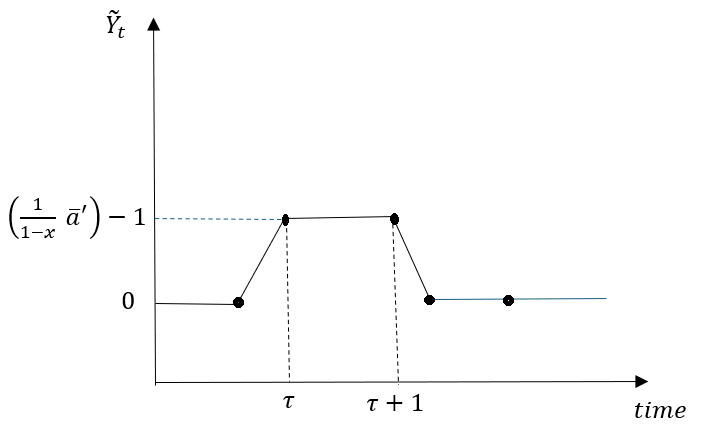
\includegraphics[scale=0.5]{y_c}
\end{figure}

\begin{figure}[H]
\centering
\caption*{$\: \: \: \: \: $ Inflation}
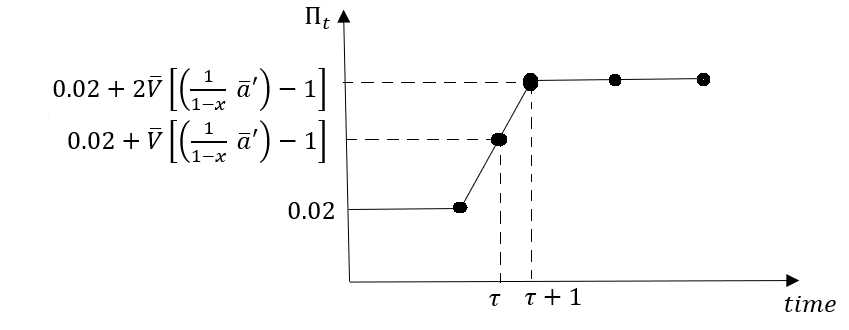
\includegraphics[scale=0.5]{timec}
\end{figure}
\end{enumerate}
\vspace{0.2in}
\noindent Assume that $b_T<1$.  If we assume that the government budget is balanced when output is at its potential level (i.e. $\widetilde{Y}_t=0$), we can write the fiscal surplus that results from government expenditure changes as follows ($S<0$ is a deficit):
\begin{eqnarray*}
S=b_T \: (Y_t-\overline{Y})-(\overline{G}'-\overline{G})  
\end{eqnarray*}
\begin{enumerate}[label=(\alph*)]
\setcounter{enumi}{4}
\item (4 points) Solve for government budget surplus as a function of $b_T$, $\overline{G}$, $\overline{G}'$ and the multiplier [\textbf{Hint:} The only difference between $Y_t$ and $\overline{Y}$, is that $Y_t$ is a function of $\overline{G}'$ and $\overline{Y}$ is a function of $\overline{G}$] \\
\\
\textbf{Answer:}\\
\begin{eqnarray*}
S=b_T (Y_t-\overline{Y})-(\overline{G}'-\overline{G}) \\[2ex]
\overline{Y}=\frac{1}{1-x}\left[a_c+a_i-b_i \: R_t+\overline{G}+\overline{X}-\overline{M}\right] \\[2ex]
Y_t=\frac{1}{1-x}\left[a_c+a_i-b_i \: R_t+\overline{G}'+\overline{X}-\overline{M}\right]  \\[2ex]
\text{So,} \: \: S=\left(\frac{b_T}{1-b_c+b_c \: b_T}- 1\right) \: \left(\overline{G}'-\overline{G}\right)
\end{eqnarray*}

\item (7 points) Using graphs showing how the government fiscal surplus responds over time, analyze how the shock in part $d$ affects the government budget. \\
\\
\textbf{Answer:}\\
When $b_T<1$ and $b_c<1$, $\frac{b_T}{1-b_c+b_c \: b_T}<1$. Therefore, 
\begin{figure}[H]
\centering
\caption*{$\: \: \: \: \: $ Government Budget}
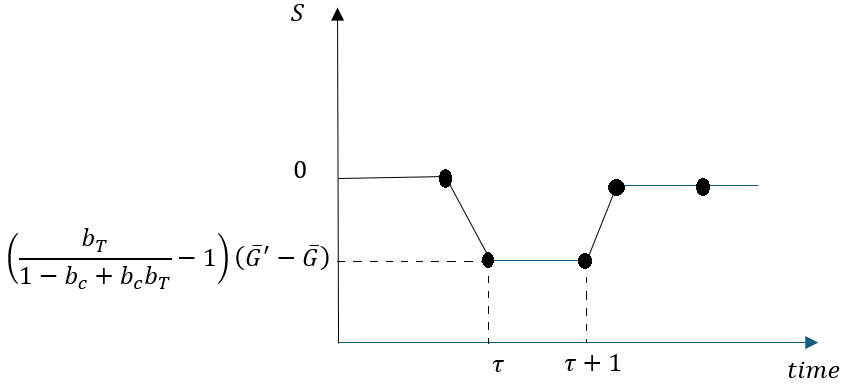
\includegraphics[scale=0.5]{gov_budget}
\end{figure}



\end{enumerate}   


\section*{Question IV: IS-MP and Phillips Curve}
Suppose that inflation at time $t$ is given by the following equation:
\begin{eqnarray*}
\pi_t=\pi^e_t+\overline{v} \: \: \: \widetilde{Y}_t+\overline{o}_t
\end{eqnarray*} 
where all the variables are the same as in the lectures. However, unlike in lectures, assume that $\pi^e_t=0.02$. That is, people expect the inflation rate to equal $2\%$ in every period.
\begin{enumerate}[label=(\alph*)]
\item (10 points) Using a version of the Phillips curve with $(\pi_t-\pi^e_t)$ on the vertical axis and a graph showing how inflation responds over time, analyze the effect of a one time price shock to the economy.\\
\\
\textbf{Answer:}\\
From the two graphs below we can see that, when people expect the inflation rate to be $2\%$ every period, price shocks have only a one-period effect on inflation.
\begin{figure}[H]
\centering
\caption*{Price shocks in an economy with no memory}
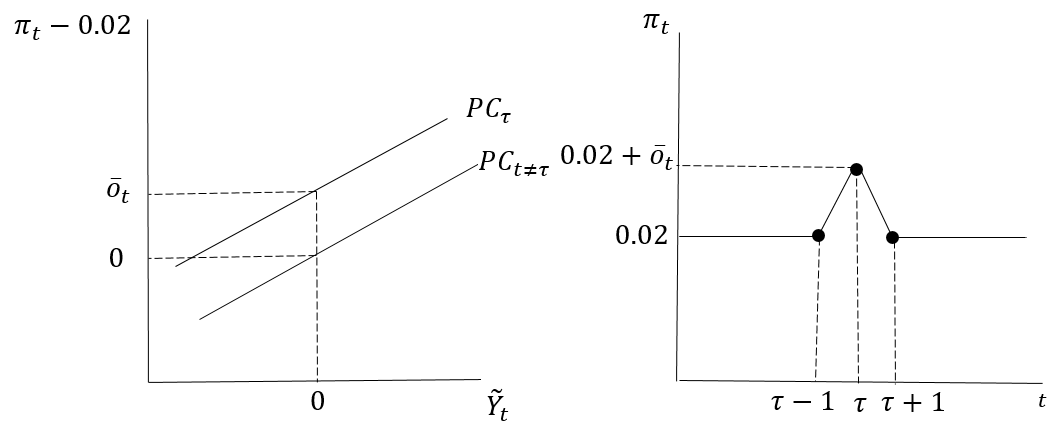
\includegraphics[scale=.65]{CB_independence}
\end{figure} 
\item (5 points) The Bank of Canada has a specific mandate to keep inflation around $2\%$. Given your answer to part a) and our discussion in class, explain the importance that this mandate is a credible commitment.
 \\
\\
\textbf{Answer:}\\
In class, when $\pi^e_t=\pi_{t-1}$, a one-time price shock changes inflation for all future preiods. If government wants to return the inflation rate to what it was before the price shock, it has to change output through monetary or fiscal policy. This means inducing recessions after positive price shocks. When a government has a credible commitment to a specific inflation target, a one-time price shock does not change expectations of future inflation. Therefore, in this case price shocks have only a transitory effect on inflation.  
\end{enumerate}

\section*{Question V: The AS-AD Model}
Consider the following economy:
\begin{eqnarray*}
\begin{array}{ll}
\text{Aggregate Expenditure} & E_t=C_t+I_t+G_t+X_t-M_t \\[1.4ex]
\text{Consumption} & C_t=a_c+b_c Y_t \\[1.4ex]
\text{Investment} & I_t=a_i-b_i \: \: \: R_t \\[1.4ex]
\text{Inflation} & \pi_t=\pi^e_t+\overline{v} \: \: \: \widetilde{Y}_t+\overline{o}_t  \\[1.4ex]
\text{Policy Rule} & R_t-\overline{r}=\overline{m}(\pi_t-\overline{\pi})  \\[1.4ex]
\text{Government Expenditure and Trade} & G_t=\overline{G}, \: \: \: \: \: \: M_t=\overline{M}, \: \: \: \: \: \: X_t=\overline{X}
\end{array}
\end{eqnarray*}
Use the previous equations to answer the following questions:
\begin{enumerate}[label=(\alph*)]
\item (5 points) Derive the AD curve. \\
\\
\textbf{Answer:}\\
As in class the AD curve is:
\begin{eqnarray*}
\widetilde{Y}_t=\frac{1}{1-b_c}\left[\overline{a}-\overline{b}_i \: \overline{m}(\Pi_t-\overline{\Pi})\right]-1
\end{eqnarray*}
\item (10 points) Assume that $\pi^e_t=\pi_{t-1}$. Suppose the economy is at its potential output equilibrium with a constant $\overline{\pi}$ inflation rate. Using the AS-AD model, carefully explain what happens to the economy \textbf{over time} if there is a one-period positive demand shock.\\
\\
\textbf{Answer:}\\
Consider a one-time demand shock at $t=\tau$:
\begin{itemize}
\item at $t=\tau$ (move from AD to AD', 0 to $\widetilde{Y}_1$, and $\overline{\Pi}$ to $\Pi_1$ in the graph below):
\begin{eqnarray*}
\begin{array}{l}
\widetilde{Y}_{\tau}=\frac{1}{1-b_c}\left[\overline{a}' -\overline{b}_i \: \overline{m}(\Pi_{\tau}-\overline{\Pi})\right]-1>0 \\[1.2ex]
\Pi_{\tau}=\overline{\Pi}+\overline{v}\: \: \widetilde{Y}_{\tau} >\overline{\Pi}
\end{array}
\end{eqnarray*}
The initial positive shock to demand increases inflation, which forces the CB to increase real interest rates . Though the CB's policy response decreases the impact of the demand shock, it does not completely offset the increase in output above its potential level. The result is that both inflation and deviations from potential output are above their long-run equilibrium.
\item  at $t=\tau+1$ (move from AD' back to AD, AS to AS',  $\widetilde{Y}_1$ to  $\widetilde{Y}_2$, and $\Pi_1$ to $\Pi_2$ in the graph below):
\begin{eqnarray*}
\begin{array}{l}
\widetilde{Y}_{\tau+1}=\frac{1}{1-b_c}\left[-\overline{b}_i \: \overline{m}(\Pi_{\tau+1}-\overline{\Pi})\right]  < 0 \\[1.2ex]
\Pi_{\tau+1}=\Pi_{\tau}+\overline{v}\: \: \widetilde{Y}_{\tau+1}\underset{>\overline{\Pi}}{<\Pi_{\tau}}
\end{array}
\end{eqnarray*}
In the period after the shock, the AD curve returns to its benchmark AD curve, and the AS curve shifts up due to the increase in the previous period inflation rate. Given that inflation rate is still above its target, the deviation from potential output is negative because the CB sets the real interest rate above its long-run level. This results in a decrease of inflation from the previous period.
\item at $t>\tau+1$ (move from AS' closer and closer to the benchmark AS curve)
\begin{eqnarray*}
\begin{array}{l}
\widetilde{Y}_{t}=\frac{1}{1-b_c}\left[-\overline{b}_i \: \overline{m}(\Pi_{t}-\overline{\Pi})\right]\underset{< 0}{>\widetilde{Y}_{t-1}}\\[1.2ex]
\Pi_{t}=\Pi_{t-1}+\overline{v}\: \: \widetilde{Y}_{t} \underset{>\overline{\Pi}}{<\Pi_{t-1}}
\end{array}
\end{eqnarray*}
\end{itemize}


\begin{figure}[H]
\centering
\caption*{$\: \: \: \: \: $ AS-AD}
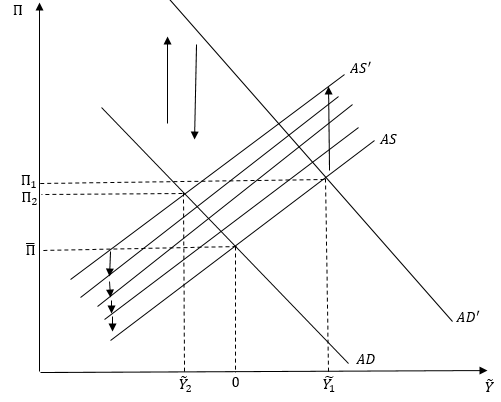
\includegraphics[scale=1]{nq_4}
\end{figure}
\end{enumerate}

\end{document}